\providecommand{\setflag}{\newif \ifwhole \wholefalse}
\setflag
\ifwhole\else

% Typography and geometry ----------------------------------------------------
\documentclass[letterpaper]{scrbook}
\usepackage[inner=3cm,top=2.5cm,outer=3.5cm]{geometry}

\renewcommand\familydefault{bch}
\usepackage[utf8]{inputenc}
\usepackage{microtype}
\usepackage[small]{caption}
\usepackage[small]{titlesec}
\raggedbottom

% Graphics -------------------------------------------------------------------
\usepackage[pdftex]{graphicx}
\graphicspath{{_include/}}
\DeclareGraphicsExtensions{.png,.pdf}

% Code formatting ------------------------------------------------------------
\usepackage{fancyvrb}
\usepackage{courier}
\usepackage{listings}
\usepackage{color}
\usepackage{alltt}


\definecolor{comment}{rgb}{0.60, 0.60, 0.53}
\definecolor{background}{rgb}{0.97, 0.97, 1.00}
\definecolor{string}{rgb}{0.863, 0.066, 0.266}
\definecolor{number}{rgb}{0.0, 0.6, 0.6}
\definecolor{variable}{rgb}{0.00, 0.52, 0.70}
\lstset{
  basicstyle=\ttfamily,
  keywordstyle=\bfseries, 
  identifierstyle=,  
  commentstyle=\color{comment} \emph,
  stringstyle=\color{string},
  showstringspaces=false,
  columns = fullflexible,
  backgroundcolor=\color{background},
  mathescape = true,
  escapeinside=&&,
  fancyvrb
}
\newcommand{\code}[1]{\lstinline!#1!}
\newcommand{\f}[1]{\lstinline!#1()!}



% Links ----------------------------------------------------------------------

\usepackage{hyperref}
\definecolor{slateblue}{rgb}{0.07,0.07,0.488}
\hypersetup{colorlinks=true,linkcolor=slateblue,anchorcolor=slateblue,citecolor=slateblue,filecolor=slateblue,urlcolor=slateblue,bookmarksnumbered=true,pdfview=FitB}
\usepackage{url}

% Tables ---------------------------------------------------------------------
\usepackage{longtable}
\usepackage{booktabs}

% Miscellaneous --------------------------------------------------------------
\usepackage{pdfsync}
\usepackage{appendix}

\usepackage[round,sort&compress,sectionbib]{natbib}
\bibliographystyle{plainnat}


\title{ggplot2}
\author{Hadley Wickham}

\begin{document}
\fi


% SET_DEFAULTS
%   GG-WIDTH: 4  GG-HEIGHT: 4
%   TEX-WIDTH: 0.5\textwidth COL: 2 
%   INLINE: FALSE
%   CACHE: TRUE
% 

% END

\chapter{Polishing your plots for publication}
\label{cha:polishing}

In this chapter you will learn how to prepare polished plots for publication.  Most of this chapter focusses on the theming capability of \ggplot which allows you to control many non-data aspects of plot appearance, but you will also learn how to adjust geom, stat and scale defaults, and the best way to save plots for inclusion into other software packages.  Together with the next chapter, manipulating plot rendering with \code{grid}, you will learn how to control every visual aspect of the plot to get exactly the appearance that you want.

The visual appearance of the plot is determined by both data and non-data related components.  Section~\ref{sec:themes} introduces the theme system which controls all aspects of non-data display.

By now you should be familiar with the many ways that you can alter the data related components of the plot---layers and scales---to visualise your data and change the appearance of the plot.  In Section~\ref{sec:theme-scale-geom} you will learn how you can change the defaults for these, so that you do not need to repeat the same parameters again and again.

Finally, Section~\ref{sec:saving} concludes the chapter with a discussion about how to get your graphics out of R and into \LaTeX, Word or other presentation or word-processing software.

\section{Themes} 
\label{sec:themes}

The appearance of non-data elements of the plot are controlled by the theme system.  They do not affect how the data is rendered by geoms, or how it is transformed by scales.  Themes don't change the perceptual properties of the plot, but they do help you customise the plot to be aesthetically pleasing or match existing style guides.  Themes give you control over the things like the  fonts in all parts of the plot: the title, axis labels, axis tick labels, strips, legend labels and legend key labels; and the colour of ticks, grid lines, and backgrounds (panel, plot, strip and legend).

This separation into data and non-data components is quite different from base and lattice graphics.  In base and lattice graphics, most functions take a very large number arguments that specify the finer points of appearance, which can make the functions complicated and hard to understand.  \ggplot takes a different approach: when creating the plot you determine how the data is display, then {\em after} it has been created you can edit every detail of the rendering, using the theming system.  \noindent Figure~\ref{fig:themes} shows some of the effects of changing the theme of a plot.  The two examples show the two themes included by default in \ggplot.

% FIGURE
%  LABEL: themes
%  CAPTION: The effect of changing themes.  \Leftc the default grey theme with
%  grey background and white gridlines.  \Rightc the alternative black and 
%  white theme with white background and grey gridlines.  Notice how the 
%  bars, data elements, are identical in both plots.
% 
% qplot(rating, data=movies, geom="histogram", binwidth=1)
% last_plot() + theme_bw()
\input{_include/c0f2afac2b11b85c988b2dd46a272b98.tex}
% END

Like many other areas of \ggplot, themes can be controlled on multiple levels from the very coarse to the very fine:

\begin{itemize}
  \item Use a built-in theme.  This affects every element of the plot in a visually consistent manner.  The default theme uses a grey panel background with white gridlines, while the alternative theme uses a white background with grey gridlines.  \secref{sec:built_in}.

  \item Modify a single element of a built-in themes. Each theme is made up of multiple elements The theme system comes with a number of built-in element rendering functions with a limited set of parameters.  By adjusting these parameters you can control things like text size and colour, background and grid line colours and text orientation.  By combining multiple elements you can create your own theme.
  
  \item Write a custom element function with grid.  This allows you to absolutely customise the appearance of every element - you are not restricted to a fixed set of drawing options.  \secref{sec:theme_elements}

  \item Use grid to alter a single item on the plot.  Using grid, the underlying drawing system, gives you the ability to alter any element drawn on the plot.  However, it comes at a cost of requiring a much deeper understand of how the plot is drawn.  This is described in Chapter~\ref{cha:grid}.
  
\end{itemize}

\noindent Generally each of these theme settings can be applied globally, to all plots, or locally to a single plot.  How to do this is described individually for each section.

\subsection{Built-in themes}
\label{sec:built_in}

There are two built-in themes.  The default, \f{theme_gray}, uses a very light grey background with white gridlines.  This follows from the advice of \citet{tufte:2006,tufte:1990,tufte:2001,tufte:1997} and \citet{brewer:1994,carr:2002,carr:1994,carr:1999}. We can still see the gridlines to aid in the judgement of position \citep{cleveland:1993a}, but they have little visual impact and we can easily ``tune'' them out. The grey background gives the plot a similar colour (in a typographical sense) to the remainder of the text, ensuring that the graphics fit in with the flow of a text without jumping out with a bright white background. Finally, the grey background creates a continuous field of colour which ensures that the plot is perceived as a single visual entity. 

The other built-in theme, \f{theme_bw}, has a more traditional white background with dark grey grid lines.  Figure~\ref{fig:themes} show some of the difference between these themes.

Both themes have a single parameter, \code{base_size}, which controls the base font size.  The base font size is the size that the axis titles use: the plot title is 20\% bigger, and the tick and strip labels are 20\% smaller.  If you want to control these sizes separately, you'll need to modify the individual elements as described in the following section.

You can apply themes in two ways:

\begin{itemize}
  \item Globally, affecting all plots when they are drawn: \code{set_theme(theme_grey())} or \code{set_theme(theme_bw())}.  \f{theme_set} returns the previous theme so that you can restore it later if you want.
  
  \item Locally, for an individual plot:  \code{qplot(...) + theme_grey()}.  A locally applied theme will override the global default.
\end{itemize}

\noindent The following example shows a few of these combinations:

% INTERWEAVE
% 
% histogram <- qplot(rating, data=movies, geom="histogram", binwidth=1)
% previous_theme <- theme_set(theme_bw())
% 
% # Themes affect the plot when they are drawn, not when they are created
% histogram
% 
% # Override the theme for a single plot by adding it on
% histogram + theme_bw(30)
% 
% # Apply the original theme to a single plot
% histogram + previous_theme
% 
% # Permanently restore the original theme
% theme_set(previous_theme)
\input{_include/346905de2684e05ec73594ea9342d814.tex}
% END

\subsection{Theme elements}
\label{sec:theme_elements}

A theme is made up of multiple \emph{elements} which control the appearance of a single item on the plot.  To get more control over appearance than given by the default themes (or to create your own theme), you can modify these elements.  Each element draws a certain type of graphical object, like text or lines. Table~\ref{tbl:elements} lists all of the customisable elements in a plot. The following two sections describe the built-in element functions, or if those don't meet your needs, how to write your own with \code{grid}.


\begin{table}
  \begin{center}
  \begin{tabular}{lll}\\
    \toprule
    Theme element              & Type     & Description  \\
    \midrule                              
    \texttt{axis.line}         & segment  & Line along axis  \\
    \texttt{axis.text.x}       & text     & x axis label  \\
    \texttt{axis.text.y}       & text     & y axis label  \\
    \texttt{axis.ticks}        & segment  & axis tick marks  \\
    \texttt{axis.ticks.y}      & segment  & axis tick marks  \\
    \texttt{axis.title.x}      & text     & horizontal tick labels  \\
    \texttt{axis.title.y}      & text     & vertical tick labels  \\[0.5em]
    \texttt{legend.background} & rect     & background of legend  \\
    \texttt{legend.key}        & rect     & background underneath legend keys \\
    \texttt{legend.text}       & text     & legend labels  \\
    \texttt{legend.title}      & text     & legend name  \\[0.5em]
    \texttt{panel.background}  & rect     &   \\
    \texttt{panel.border}      & rect     &   \\
    \texttt{panel.grid.major}  & line     & major grid lines \\
    \texttt{panel.grid.minor}  & line     & minor grid lines \\[0.5em]
    \texttt{panel.empty}       & rect     & panel with no data   \\
    \texttt{plot.background}   & rect     & background of the entire plot \\
    \texttt{plot.title}        & text     & plot title   \\[0.5em]
    \texttt{strip.background}  & rect     &   \\
    \texttt{strip.text.x}      & text     & text for horizontal strips  \\
    \texttt{strip.text.y}      & text     & text for vertical strips  \\
    \bottomrule                           
  
  \end{tabular}
  \end{center}
  \caption{Theme elements}
  \label{tbl:elements}
\end{table}

There are three elements that have individual \code{x} and \code{y} settings: \code{axis.text}, \code{axis.title} and \code{strip.text}.  Having a different setting for the horizontal and vertical elements allows you to control how text should appear in different orientations.

There are four basic types of built element functions.

\begin{itemize}
  \item \code{theme_text}. family, face, colour, size, hjust, vjust, angle, lineheight

  \item \code{theme_line} and \code{theme_segment}.  Lines and segments have the same options but are drawn in a slightly different way.  Make sure you match the appropriate type or you will get strange grid errors.  colour, size, linetype

  \item \code{theme_rect}, fill, colour, size, linetype

  \item \code{theme_blank}.  Use this element type if you don't want anything drawn, or any space allocated for that element.  

\end{itemize}

Again there are two ways to set individual elements, globally or locally:

\begin{itemize}
  \item \f{theme_update} modifies the global theme: \code{theme_update(plot.title = theme_text(colour = "red"))}.
  
  \item \f{opts} modifies the local theme: \code{qplot(...) + opts(plot.title = theme_text(colour = "red"))}.
  
\end{itemize}

% EXAMPLES
% 
% Change angle of axis labels
% 

\subsection{More advanced control}
\label{sub:more_advanced_control}

You can also write your own custom element functions.  You'll need to know more about grid to do this, so this is described in Section~\ref{sec:element-functions}.

\section{Customising scales and geoms}
\label{sec:theme-scale-geom}

When producing a consistent theme, you may also want to tune some of the scale and geom defaults.  Rather than having to manually specify the changes every time you add the scale or geom, you can use the following functions to alter the default settings for scales and geoms.

\subsection{Scales}
\label{sub:customise-scales}

To change the default scale associated with an aesthetic, use \f{set_default_scale}. (See Table~\ref{tbl:default-scales} for the defaults.)  This function takes three arguments: the name of the aesthetic, the type of variable (discrete or continuous) and the name of the scale to use as the default.  Further arguments override the default parameters of the scale.  The following example sets up colour and fill scales for black and white printing:

% INTERWEAVE
% 
% set_default_scale("colour", "discrete", "grey")
% set_default_scale("fill", "discrete", "grey")
% set_default_scale("colour", "continuous", "gradient", 
%   low = "white", high = "black")
% set_default_scale("fill", "continuous", "gradient", 
%   low = "white", high = "black")
\input{_include/7e79182ad9d19098cfab168d90648015.tex}
% END

\subsection{Geoms and stats}
\label{sub:geoms_and_stats}

You can customise geoms and stats in a similar way with \f{update_geom_defaults} and \f{update_stat_defaults}.  The following example demonstrates changing the default point colour and changing the default histogram to a density (``true'') histogram.

Table~\ref{tbl:geom-defaults} lists all of the common aesthetic defaults.  If you change one, it's a good idea to change all the other that you use to ensure that your plots look consistent.  See Chapter~\ref{cha:specifications} for how the values are interpreted by R.

% aes_value <- function(x) paste(names(x), x, sep =": ")
% 
% geoms <- Geom$find_all()
% aes_defaults <- lapply(geoms, function(y) aes_value(y$default_aes()))
% names(aes_defaults) <- unname(sapply(geoms, function(y) y$objname))
% aes_list <- invert(aes_defaults)
% aes_list <- Filter(function(x) length(x) > 1, aes_list)
% aes_names <- lapply(aes_list, function(x) paste(sort(x), collapse = ", "))
% tabulate(data.frame(names(aes_names), unlist(aes_names)))

\begin{table}
  \begin{center}
  \begin{tabular}{llp{4in}}
    \toprule
    Aesthetic & Default value & Geoms \\
    \midrule
    colour & \#3366FF & contour, density\_2d, quantile, smooth                                                                                                                                                                \\
     & NA      & area, bar, histogram, polygon, rect, tile                                                                                                                                                            \\
     & black   & abline, crossbar, density, errorbar, hline, jitter, line, linerange, path, point, pointrange, rug, segment, step, text, vline                                                                        \\
     & grey60  & boxplot, ribbon                                                                                                                                                                                      \\
    fill & NA        & crossbar, density, jitter, point, pointrange                                                                                                                                                         \\
     & grey60    & area, bar, histogram, polygon, rect, ribbon, smooth, tile                                                                                                                                            \\
    intercept & 0    & abline, hline, vline                                                                                                                                                                                 \\
    linetype & 1     & abline, area, bar, contour, crossbar, density, density\_2d, errorbar, histogram, hline, line, linerange, path, pointrange, polygon, quantile, rect, ribbon, rug, segment, smooth, step, tile, vline   \\
    shape & 19       & jitter, point, pointrange                                                                                                                                                                            \\
    size & 0.5       & abline, area, bar, boxplot, contour, crossbar, density, density\_2d, errorbar, histogram, hline, line, linerange, path, pointrange, polygon, quantile, rect, ribbon, rug, segment, smooth, step, vline\\
     & 2         & jitter, point                                                                                                                                                                                        \\
    weight & 1       & bar, boxplot, contour, density, density\_2d, histogram, quantile, smooth                                                                                                                              \\
  \bottomrule
  \end{tabular}
  \end{center}
  \caption{Default aesthetic values for geoms.  See Chapter~\ref{cha:specifications} for how the values are interpreted by R.}
  \label{tbl:geom-defaults}
\end{table}


% INTERWEAVE
% 
% update_geom_defaults("point", aes(colour = "darkblue"))
% qplot(mpg, wt, data=mtcars)
% # update_stat_defaults("bin", aes(y = ..density..), binwidth = 1)
% qplot(rating, data=movies, geom="histogram", binwidth=1)
\input{_include/5b2dbe0c7bf07635d822df51e228ad8f.tex}
% END

\section{Saving your output}
\label{sec:saving}

For interactive use, \f{ggsave}, will use the size of the current graphics device (useful for ensuring a good aspect ratio), but when creating final versions it's recommended to set width and height so that all graphics for a document are the same size.

You have two basic choices of output: raster or vector.  Vector graphics are procedural: .  This means that they are essentially ``infinitely'' zoomable - there is no loss of detail.  Raster graphics are stored as an array of pixels.  Fixed resolution.  Generally, vector output is more desirable, but for complex graphics containing thousands of graphical objects it can be slow to render.  In this case, it may be better to switch to raster output.  For printed use, a high-resolution (e.g. 600 dpi) graphic may be an acceptable compromise, but can be large.

\begin{figure}[htbp]
  \centering
    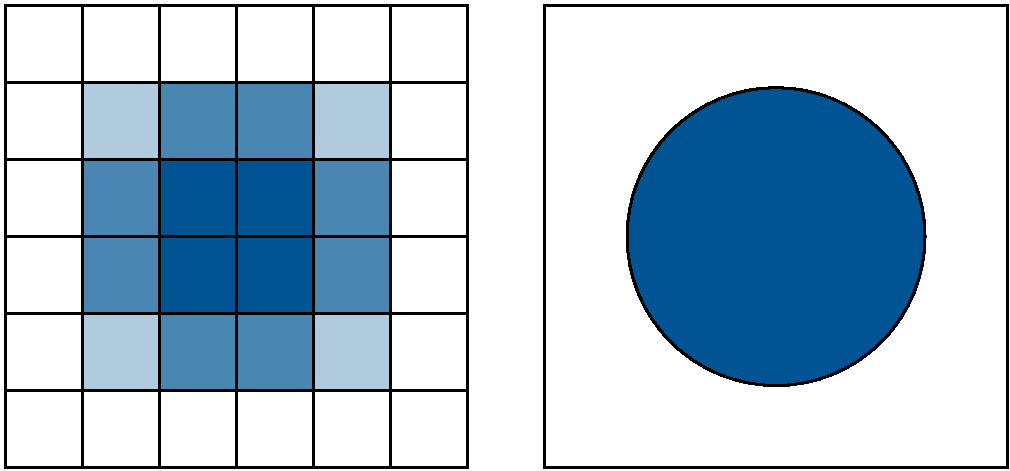
\includegraphics[width= 0.5\textwidth]{vector-raster}
  \caption{The difference between raster, {\it left}, and vector, {\it right}, graphics. }
  \label{fig:vector-raster}
\end{figure}

Table~\ref{tbl:graphic-recommendation} lists recommended graphic formats for various tasks.  R output generally works best as part of a *nix development tool chain: using png or pdf output in \LaTeX documents.  With Microsoft Office things are little more complicated.  You have two choices of vector output neither of which are perfect.  The first option is to use Windows meta files (\code{wmf}), which are supported natively by Office but do not support transparency.  {\sc pdf}s do support transparency, but when included into a Office do not.

If you are using \LaTeX, I recommend including \verb|\DeclareGraphicsExtensions{.png, .pdf}| in the preamble.  Then you don't need to specify the file extension in \verb|includegraphics| commands, but \LaTeX will pick png files in preference to pdf.  I choose this order because you can produce all your files in pdf, and then go back and re-render any big ones as pngs.

\begin{table}
  \begin{center}
  \begin{tabular}{lll}
    \toprule
    Graphics device & Type & Recommended for \\
    \midrule
    pdf   & vector & pdflatex\\
    ps    & vector & latex \\
    wmf   & vector & MS office \\
    png   & raster & web, pdflatex \\
    tiff  & raster & some publishers \\
    \bottomrule 
  \end{tabular}
  \end{center}
  \caption{Recommended graphic output for different purposes.}
  \label{tbl:graphic-recommendation}
\end{table}

\ifwhole
\else
  \nobibliography{/Users/hadley/documents/phd/references}
  \end{document}
\fi
